\subsubsection{Environments}

In this experiment,
five simulated environments were considered:
Pendulum \cite{Task_OpenAIGym},
Acrobot \cite{Task_OpenAIGym,Task_Acrobot1,Task_Acrobot2},
CartPole \cite{Task_OpenAIGym,Task_CartPole},
Door \cite{Task_Adroit},
and Hammer \cite{Task_Adroit}.
The detailed descriptions and visualizations of these environment are shown in Table \ref{ch:DAIL:tab:Tasks} and Figure \ref{ch:DAIL:fig:EnvVisualization},
respectively.
From such environments,
five domain adaptive tasks were decided,
each of which included two different environments - an expert domain and a learner domain.
These tasks can be divided into 2 categories as follows:

\begin{itemize}
  \item \textbf{Low-dimensional tasks}:
        \begin{itemize}
          \item Pendulum-Acrobot: Expert domain is Pendulum and learner domain is Acrobot.
          \item Pendulum-CartPole: Expert domain is Pendulum and learner domain is CartPole.
          \item Acrobot-CartPole: Expert domain is Acrobot and learner domain is CartPole.
        \end{itemize}
        To provide expert demonstrations,
        for each task,
        the Trust Region Policy Optimization method \cite{RL_TRPO} is first trained on the expert domain using the shaped reward signal.
        Then,
        20 expert demonstrations are collected by executing the learned policies in the expert domain simulator.
        Each demonstration includes a sequence of state-action pairs.
        It should be noted that only successful demonstrations where the learned policies can accomplish the task are collected.

  \item \textbf{High-dimensional tasks}:
        \begin{itemize}
          \item Door-Door: The expert and learner domains have different friction parameter. The friction parameter in expert domain is $[1, 1, 1]$, while in learner domain is $[4.0, 4.0, 4.0]$.
          \item Hammer-Hammer: The expert and learner domains have different mass of the hammer. The mass of the hammer in expert domain is 0.253442, while in learner domain is 1.0.
        \end{itemize}
        Twenty expert demonstrations are used for each task.
        The demonstrations are collected from humans using the Mujoco HAPTIX system \cite{Mujoco_HAPTIX} and publicly available \cite{Task_Adroit}.
\end{itemize}

\begin{landscape}
  \begin{table}[htbp!]
    \centering
    \caption{Description of five simulated environments used in the experiment.}
    \label{ch:DAIL:tab:Tasks}
    \begin{tabular}{cccp{8cm}}
  \toprule
  \textbf{Task}                                             & \textbf{State space} & \textbf{Action space} & \textbf{Description}                                                       \\
  \midrule
  Pendulum \cite{Task_OpenAIGym}                            & 3 (continuous)       & 1 (continous)         & Swinging up a pendulum.                                                    \\
  Acrobot \cite{Task_OpenAIGym,Task_Acrobot1,Task_Acrobot2} & 6 (continuous)       & 3 (discrete)          & Swinging the end of the lower link up to a given height                    \\
  CartPole \cite{Task_OpenAIGym,Task_CartPole}              & 4 (continuous)       & 2 (discrete)          & Preventing the pendulum from falling over by applying a force to the cart. \\

  Door \cite{Task_Adroit}                                   & 39 (continuous)      & 28 (continuous)       & A 24-DoF hand attempts to undo the latch and swing the door open.          \\
  Hammer \cite{Task_Adroit}                                 & 46 (continuous)      & 26 (continous)        & A 24-DoF hand attempts to use a hammer to drive the nail into the board.   \\
  \bottomrule
\end{tabular}

  \end{table}

  \begin{table}[htbp!]
    \centering
    \caption{\DAIL{} hyperparameters used in the experiment. Each number corresponds to the number of nodes in a network layer.}
    \label{ch:DAIL:tab:ModelHyperparameteres}
    
\begin{tabular}{lccc}
  \toprule
  \textbf{}              & \textbf{Feature Extractor $F$}    & \textbf{Generator $G$}                            & \textbf{Discriminator $D$}      \\
  \midrule
  Low-dimensional Tasks  & $(s^t_x, a^t_x)$ - 32 - 32 - 16   & $(\mathbf{f}_x)$ - 32 - 32 - $(a^t_\mathcal{L})$  & $(\mathbf{f}_x)$ - 32 - 32 - 1  \\
  High-dimensional Tasks & $(s^t_x, a^t_x)$ - 128 - 128 - 64 & $(\mathbf{f}_x)$ - 128 - 64 - $(a^t_\mathcal{L})$ & $(\mathbf{f}_x)$ - 128 - 64 - 1 \\
  \bottomrule
\end{tabular}

  \end{table}
\end{landscape}

\begin{figure}[htbp!]
  \centering
  \begin{subfigure}[b]{0.25\textwidth}
    \centering
    \frame{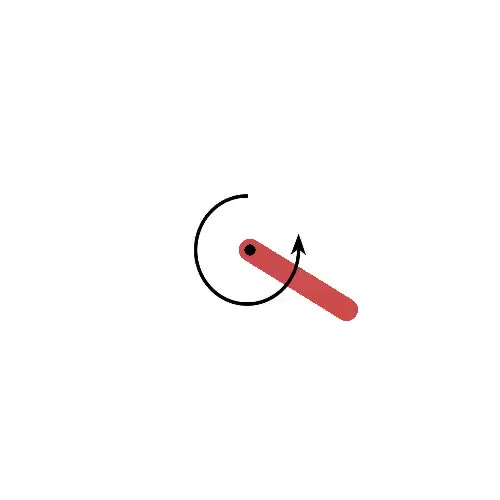
\includegraphics[width=\linewidth]{\FigsDir/Pendulum.jpg}}
    \caption{Pendulum}
  \end{subfigure}
  \hfill
  \begin{subfigure}[b]{0.25\textwidth}
    \centering
    \frame{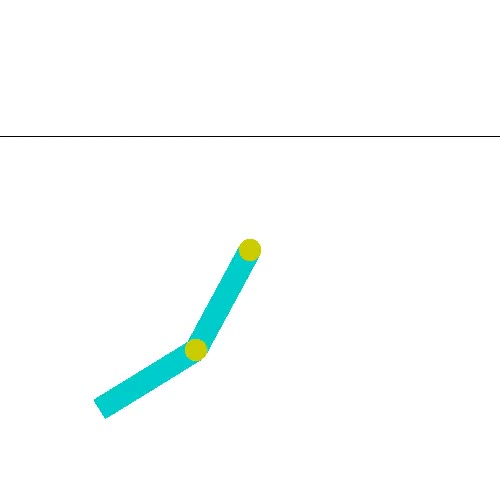
\includegraphics[width=\linewidth]{\FigsDir/Acrobot.jpg}}
    \caption{Acrobot}
  \end{subfigure}
  \hfill
  \begin{subfigure}[b]{0.25\textwidth}
    \centering
    \frame{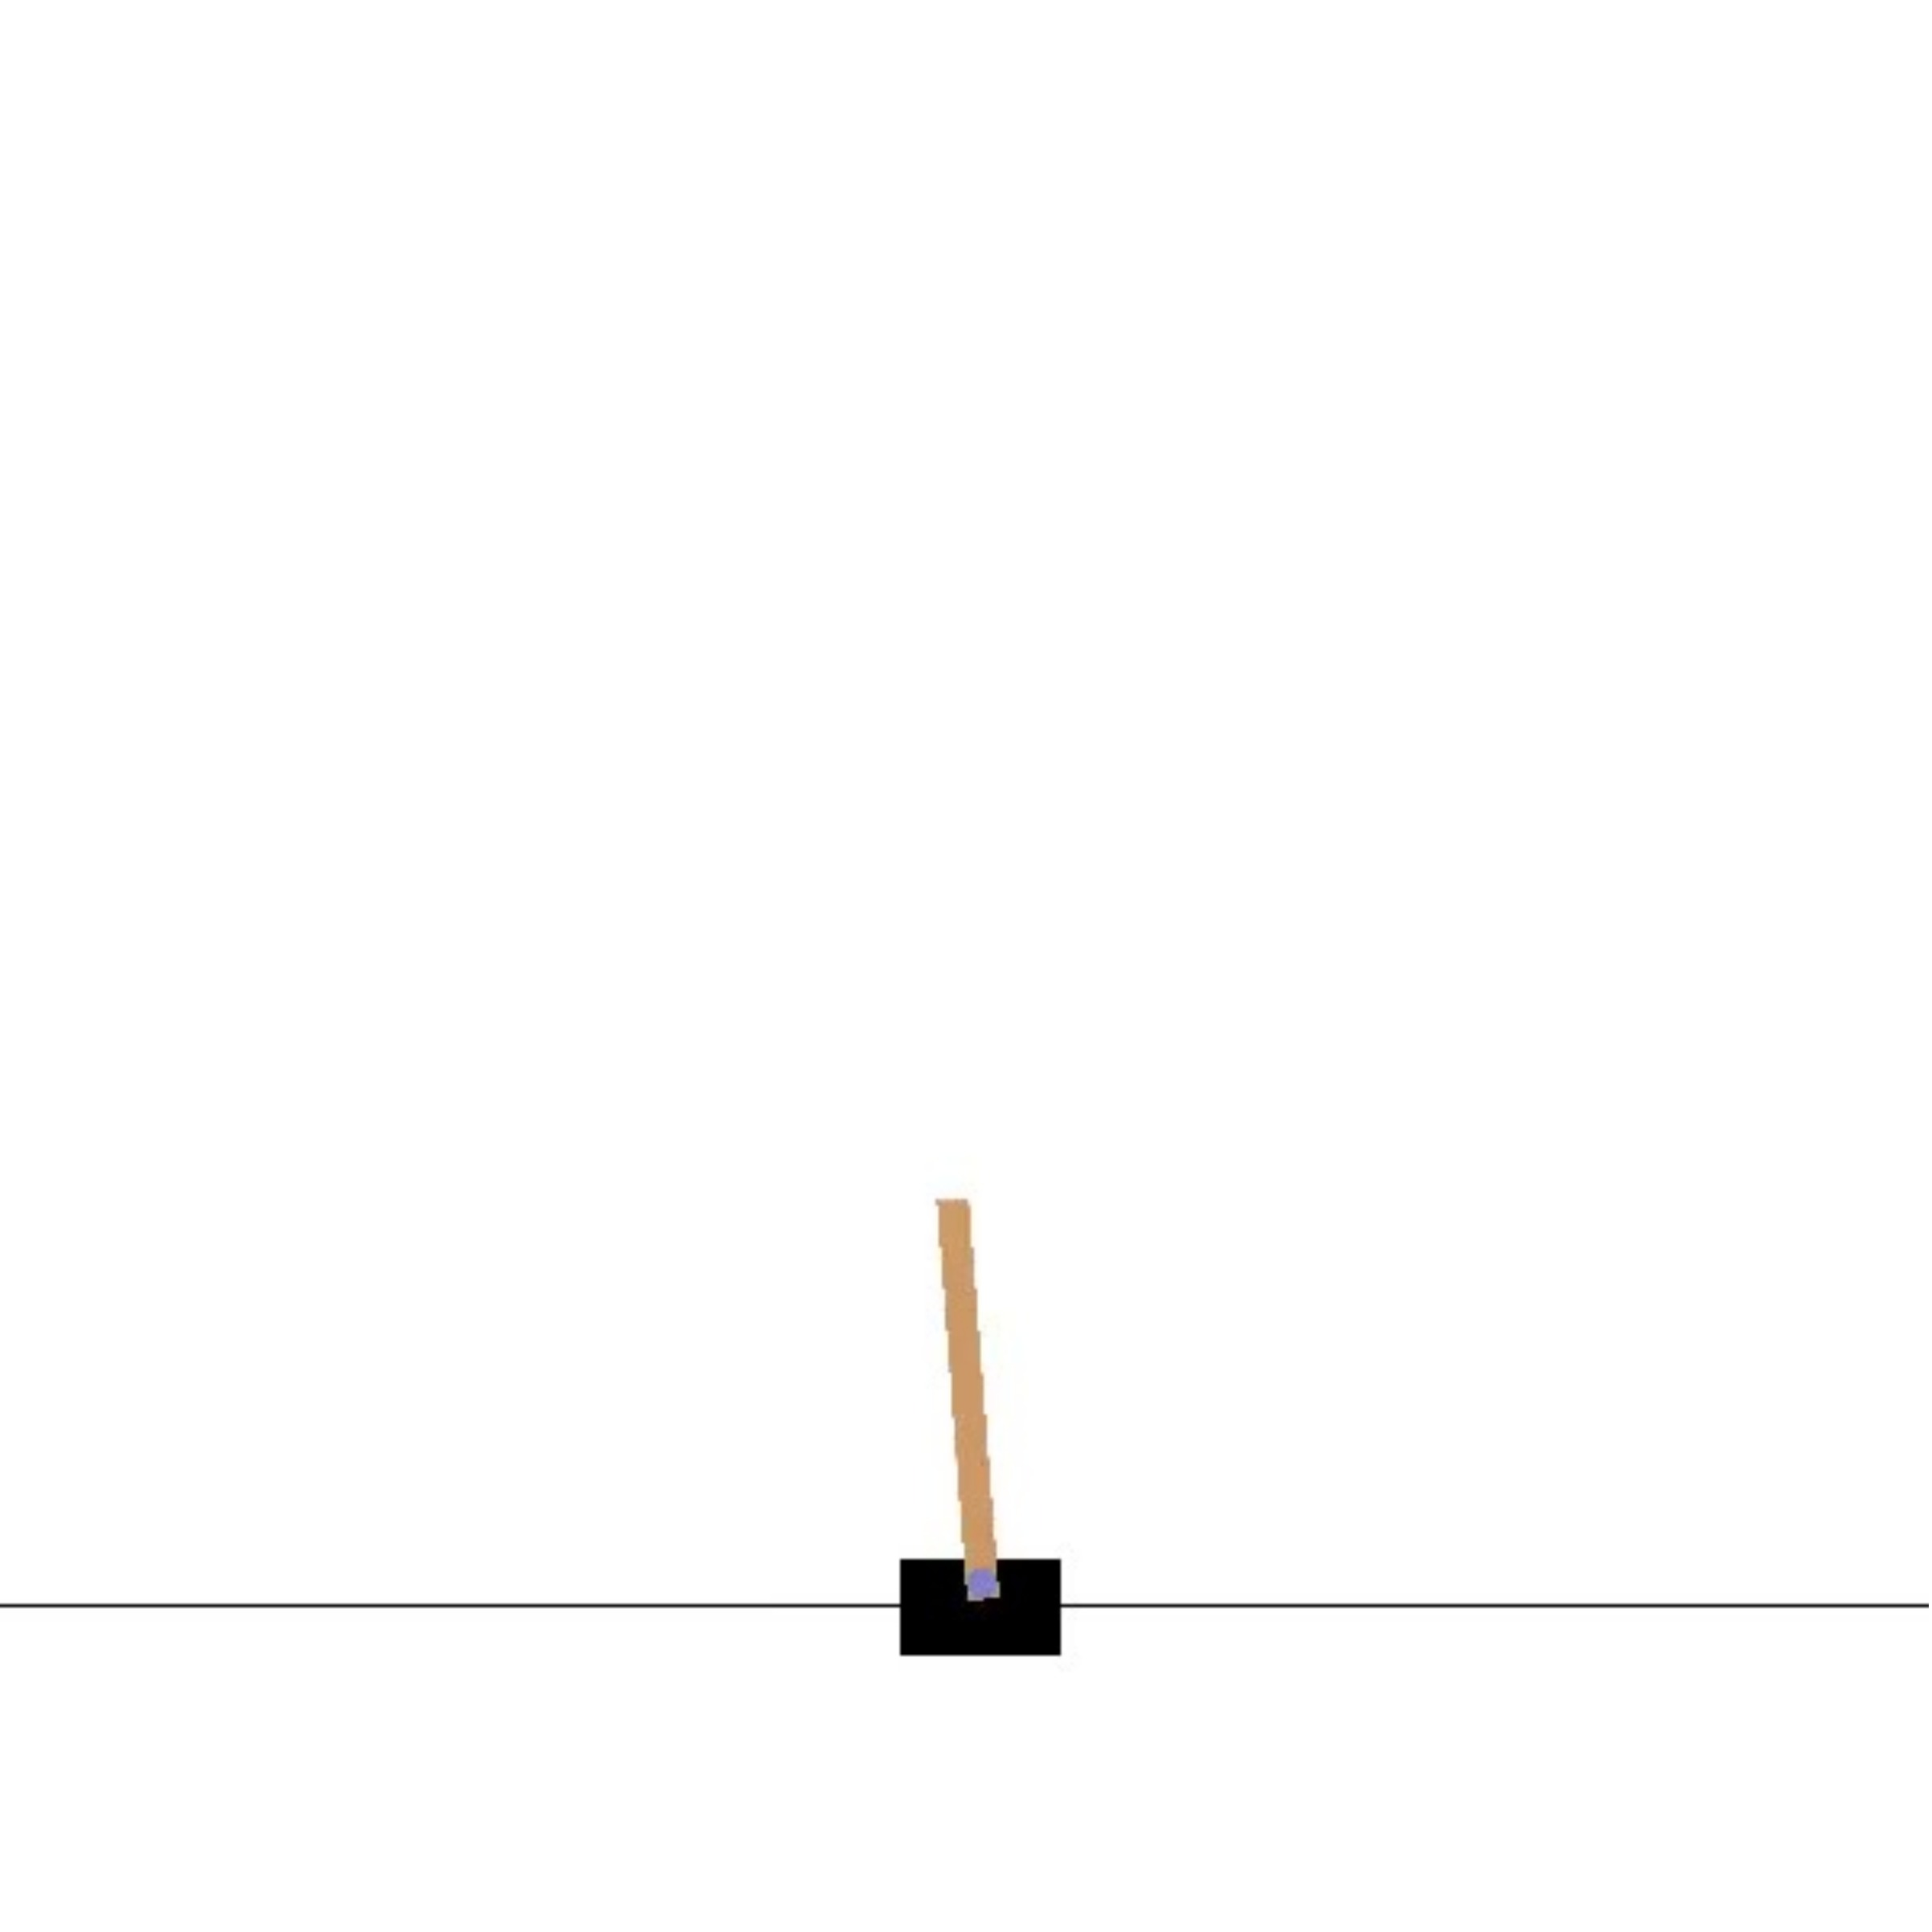
\includegraphics[width=\linewidth]{\FigsDir/CartPole.jpg}}
    \caption{CartPole}
  \end{subfigure}
  \par\bigskip
  \begin{subfigure}[b]{0.25\textwidth}
    \centering
    \frame{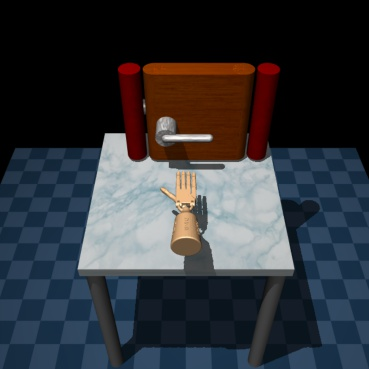
\includegraphics[width=\linewidth]{\FigsDir/Door.jpg}}
    \caption{Door}
  \end{subfigure}
  \hspace{4em}
  \begin{subfigure}[b]{0.25\textwidth}
    \centering
    \frame{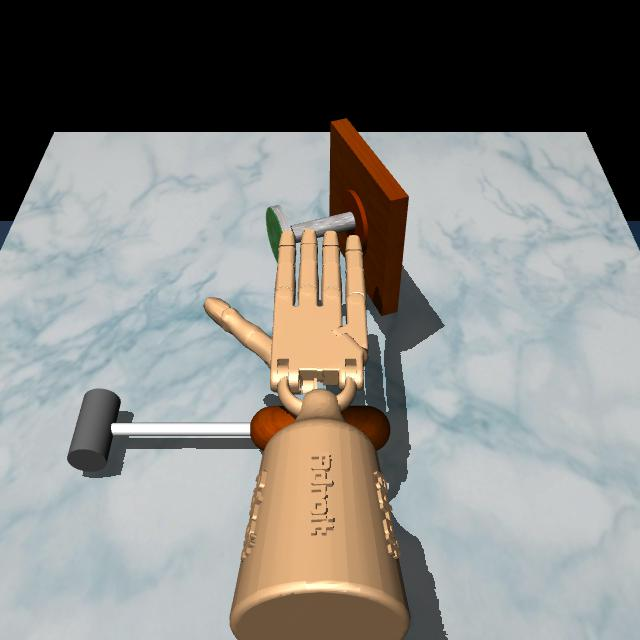
\includegraphics[width=\linewidth]{\FigsDir/Hammer.jpg}}
    \caption{Hammer}
  \end{subfigure}
  \caption{Visual rendering of five simulated environments used in the experiment.}
  \label{ch:DAIL:fig:EnvVisualization}
\end{figure}



%==================================================
\subsubsection{Baselines}

The performance of the proposed \DAIL{} agent was evaluated in comparison with the following baseline methods:

\begin{itemize}
  \item
        Trust Region Policy Optimization (TRPO) \cite{RL_TRPO} is a Reinforcement learning-based agent.
        The agent was trained directly on the learner domain and had access to the shaped reward function.
        This baseline set an upper bound for the performance of domain adaptation algorithms.

  \item
        GAMA-PA \cite{DAIL_Model_DAIL}:
        The agent introduced a two-step approach for domain adaptation in imitation learning.
        It first learns the state-action maps between expert and learner domains, and then utilizes it to learn an optimal policy.
        The agent parameters are employed as reported in \cite{DAIL_Model_DAIL} in order to ensure a fair comparison.
\end{itemize}

%==================================================
\subsubsection{Network Structure and Hyperparameters}

Deep feed-forward networks with 2 hidden layers are used for three $F$, $G$, $D$ networks of the proposed agent.
\added{Grid search was utilized in order to find an optimal set of network hyperparameters.
  Since high-dimensional tasks are more challenging compared to low-dimensional tasks,
  DAIL-GAN requires a higher number of nodes in each network layer in order to provide a high and consistent performance.}
The network hyperparameters are shown in Table \ref{ch:DAIL:tab:ModelHyperparameteres}.
In this experiment, the learning rate was 0.0003.
Adam was used as an optimizer.
